\let\negmedspace\undefined
\let\negthickspace\undefined
\documentclass[journal,12pt,onecolumn]{IEEEtran}
\usepackage{cite}
\usepackage{amsmath,amssymb,amsfonts,amsthm}
\usepackage{algorithmic}
\usepackage{graphicx}
\graphicspath{{Figs/}}
\usepackage{textcomp}
\usepackage{xcolor}
\usepackage{txfonts}
\usepackage{listings}
\usepackage{enumitem}
\usepackage{mathtools}
\usepackage{gensymb}
\usepackage{comment}
\usepackage{caption}
\usepackage[breaklinks=true]{hyperref}
\usepackage{tkz-euclide} 
\usepackage{listings}
\usepackage{gvv}                                        
%\def\inputGnumericTable{}                                 
\usepackage[latin1]{inputenc}     
\usepackage{xparse}
\usepackage{color}                                            
\usepackage{array}                                            
\usepackage{longtable}                                       
\usepackage{calc}                                             
\usepackage{multirow}
\usepackage{multicol}
\usepackage{hhline}                                           
\usepackage{ifthen}                                           
\usepackage{lscape}
\usepackage{tabularx}
\usepackage{array}
\usepackage{float}
%\newtheorem{theorem}{Theorem}[section]
%\newtheorem{theorem}{Theorem}[section]
%\newtheorem{problem}{Problem}
%\newtheorem{proposition}{Proposition}[section]
%\newtheorem{lemma}{Lemma}[section]
%\newtheorem{corollary}[theorem]{Corollary}
%\newtheorem{example}{Example}[section]
%\newtheorem{definition}[problem]{Definition}

\begin{document}

\title{9.2.35}
\author{AI25BTECH11002 - Ayush Sunil Labhade}
\maketitle
%\renewcommand{\thefigure}{\theenumi}
%\renewcommand{\thetable}{\theenumi}

\textbf{Question :} A circle S passes through the point (0, 1) and is orthogonal to the circle $\brak{x-1}^2 + y^2 =16$ and $x^2 + y^2 =1$.

\textbf{Solution :}

The general equation of the circle is 

\begin{align}
  x^2 + y^2 + d x + e y + f = 0
\end{align}

The condition for passing through \brak{0,1} is

\begin{align}
  e + f = -1
\end{align}

The orthogonality condition is $d_1$ d + $e_1$ e = 2 $\brak{f + f_1}$

For the first circle, $d_1$ = -2, $e_1$ = 0, $f_1$ = -15, yielding

\begin{align}
  -2 d = 2 \brak{f -15}
\end{align}

For the second circle, $d_1$ = 0, $e_1$ = 0, $f_1$ = -1, yielding

\begin{align}
  0 = 2 \brak{f -1}
\end{align}

The system of equations is

\begin{align}
  \augvec{3}{1}{0 & 1 & 1 & -1 \\
  -2 & 0 & -2 & -30 \\
  0 & 0 & -2 & -2}
\end{align}
Converting in its RREF, we get,
\begin{align}
  \augvec{3}{1}{0 & 1 & 1 & -1 \\
  -2 & 0 & -2 & -30 \\
  0 & 0 & -2 & -2}
\end{align}

Using RREF or solving, f = 1, d = 14, e = -2.

Thus, the equation is

\begin{align}
  x^2 + y^2 + 14x - 2y + 1 = 0
\end{align}
\begin{figure}[H]
  \centering
  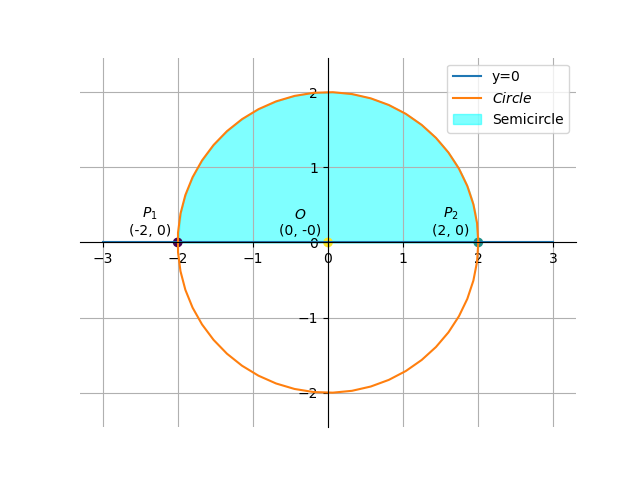
\includegraphics[width=0.7\columnwidth]{plot.png} 
   \caption*{Fig : Circle}
  \label{Fig1}
\end{figure}

\end{document}
